\documentclass[professionalfonts]{beamer}
\newif\ifita
\itatrue % comment out to hide answers
\itafalse
\usepackage[familydefault,light]{Chivo} 
\usepackage[T1]{fontenc}
\usenavigationsymbolstemplate{}
\usepackage[]{hyperref}
\usepackage{tikz,pgf,pgfarrows,pgfnodes,pgfbaseimage}
\graphicspath{{./Pics/}}
\usetikzlibrary{shapes}
\usepackage{setspace}
\newcommand{\evi}[1]{{\colorbox{yellow!50}{{#1}}}}
\newcommand{\exe}[1]{{\color{black!50}{{#1}}}}
\newcommand{\kw}[1]{{\colorbox{black!30}{\color{white}{#1}}}}
\tikzstyle{nd}=[circle,draw=black,thick,minimum size=.8cm,inner sep=1pt]
\setbeamercovered{transparent}
\usetheme{Singapore}
\tikzstyle{nodo}=[ellipse,draw=black!60,fill=black!10,line width=.7pt,minimum width=.7cm,minimum height=.4cm]
\usecolortheme[named=gray]{structure}
\setbeamercolor{block title}{bg=black!20,fg=black}
\setbeamercolor{block body}{bg=black!10,fg=black}

%%%%%%%%%%%%%%%%%%%%%
\ifita
\title{Algoritmi Numerici (Parte IV)}
\subtitle{[Lezione 1] Interpolazione Polinomiale}
\else
\title{Numerics (Part IV)}
\subtitle{[Lecture 1] Polynomial Interpolation}
\fi
\date{}
\author{Alessandro Antonucci\\{\tt alessandro.antonucci@supsi.ch}}
%%%%%%%%%%%%%%%%%%%%%%%%%%%%
\begin{document}
\maketitle
\frame{\frametitle{\ifita Un Algoritmo Migliore per Interpolazione Polinomiale \else A Better Algorithm for Polynomial Interpolation \fi}
\begin{itemize}
\item \ifita Forma alternativa per polinomio, es. \else An alternative form for the polynomial, ex.\fi 
$p_3(x)=c_0+c_1 (x-x_0) + c_2(x-x_0)(x-x_1)+c_3(x-x_0)(x-x_1)(x-x_2)$
\item $p_n(x)=\sum_{i=0}^n c_i \left[ \prod_{j=0}^{i-1} (x-x_j) \right] $
\item \ifita Impongo passaggio per gli $n+1$ punti: \else Requiring the passage through the $n+1$ points \fi
\vskip 5mm
\begin{center}
$\begin{array}{|ccccc|c|}
\hline
1 & 0 & 0 & \ldots & 0 & y_0\\ 
1 & x_1-x_0 & 0 & \ldots & 0 & y_1\\
&&\ldots&\ldots&&\\
1 & x_n-x_0 & (x_n-x_0)(x_n-x_1) & \ldots & \prod_{j=0}^{n-1} (x_n-x_j)&y_n\\
\hline
\end{array}$
\end{center}
\vskip 3mm
\item \ifita Sistema triangolare. Complessit\`a $O(n^2)$ (e non $O(n^3)$)! \else 
Triangular: quadratic (instead of cubic) complexity
\fi
\end{itemize}}


\frame{\frametitle{\ifita Metodo differenze finite \else Finite Differences Method\fi}
\begin{itemize}
\item \ifita Dati \else Data \fi $\{(x_i,y_i)\}_{i=0}^n$
\item \ifita Differenze di ordine 1: \else Order-1 Differences \fi $f[x_i]:=f(x_i)$ $\forall i=0,\ldots,n$
\item \ifita Ordine due \else Order-2 \fi $f[x_i,x_{i+1}]:= \frac{f[x_{i+1}]-f[x_i]}{x_{i+1}-x_i}$ $\forall i=0,\ldots,n-1$
\item \ifita Ordine tre \else Order-3 \fi $f[x_i,x_{i+1},x_{i+2}]:= \frac{f[x_{i+1},x_{i+2}]-f[x_i,x_{i+1}]}{x_{i+2}-x_i}$ $\forall i=0,\ldots,n-2$
\item \ifita Ordine quattro \else Order-4 \fi $f[x_i,x_{i+1},x_{i+2},x_{i+3}]:= \frac{f[x_{i+1},x_{i+2},x_{i+3}]-f[x_i,x_{i+1},x_{i+2}]}{x_{i+3}-x_i}$ $\forall i=0,\ldots,n-3$
\item \ifita Ordine $k$ \else Order-$k$ \fi = \ifita differenza fra ultima e prima ordine $k-1$ \else Difference between last and fiirst Order-$(k-1)$\fi
\ifita
diviso ultima $x$ meno prima $x$
\else
divided by difference between last and first $x$
\fi

\item \ifita Ordine $n+1$\else Order-$(n+1)$ \fi $f[x_0,x_1,\ldots,x_n]=\frac{f[x_1,\ldots,x_n]-f[x_0,\ldots,x_{n-1}]}{x_n-x_0}$
\end{itemize}
}

\frame{\frametitle{\ifita Metodo differenze finite \else Finite Differences Method \fi (ii)}
\begin{itemize}
\item \ifita Calcoli su struttura a piramide (es. $5$ punti, quindi $n=4$
\else 
Calculations on a pyramid-shaped structure (ex. 5 points, $n=4$
\fi
)
\end{itemize}
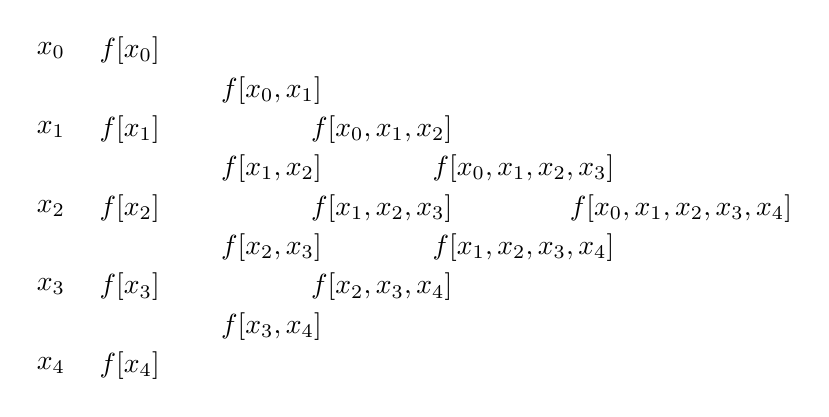
\begin{tikzpicture}
\node[] at (-1,5) {$x_0$};
\node[] at (-1,4) {$x_1$};
\node[] at (-1,3) {$x_2$};
\node[] at (-1,2) {$x_3$};
\node[] at (-1,1) {$x_4$};
\node[] at (0,5) {$f[x_0]$};
\node[] at (0,4) {$f[x_1]$};
\node[] at (0,3) {$f[x_2]$};
\node[] at (0,2) {$f[x_3]$};
\node[] at (0,1) {$f[x_4]$};
\node[] at (1.8,4.5) {$f[x_0,x_1]$};
\node[] at (1.8,3.5) {$f[x_1,x_2]$};
\node[] at (1.8,2.5) {$f[x_2,x_3]$};
\node[] at (1.8,1.5) {$f[x_3,x_4]$};
\node[] at (3.2,4) {$f[x_0,x_1,x_2]$};
\node[] at (3.2,3) {$f[x_1,x_2,x_3]$};
\node[] at (3.2,2) {$f[x_2,x_3,x_4]$};
\node[] at (5,3.5) {$f[x_0,x_1,x_2,x_3]$};
\node[] at (5,2.5) {$f[x_1,x_2,x_3,x_4]$};
\node[] at (7,3) {$f[x_0,x_1,x_2,x_3,x_4]$};
\end{tikzpicture}}

\frame{\frametitle{\ifita Metodo differenze finite \else Finite Differences Method \fi (ii)}
    \begin{itemize}
        \item \ifita Calcoli su struttura a piramide (es. $5$ punti, quindi $n=4$
        \else 
        Calculations on a pyramid-shaped structure (ex. 5 points, $n=4$
        \fi
        )
    \end{itemize}
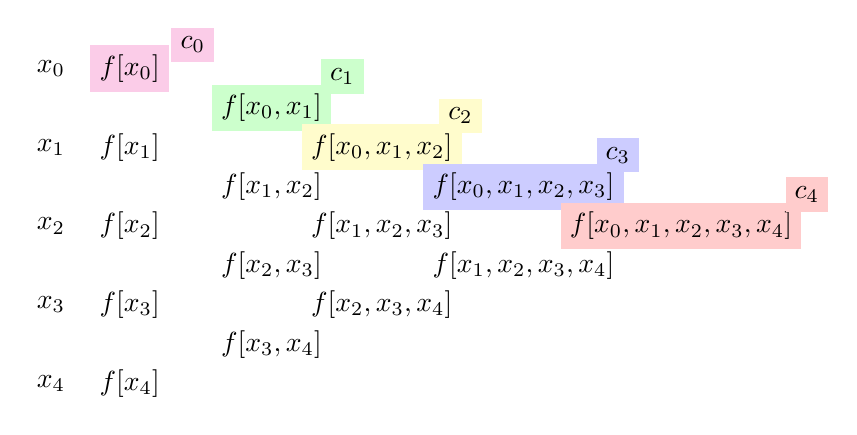
\begin{tikzpicture}
\node[] at (-1,5) {$x_0$};
\node[] at (-1,4) {$x_1$};
\node[] at (-1,3) {$x_2$};
\node[] at (-1,2) {$x_3$};
\node[] at (-1,1) {$x_4$};
\node[fill=magenta!20] at (0,5) {$f[x_0]$};
\node[fill=magenta!20] at (0.8,5.3) {$c_0$};
\node[] at (0,4) {$f[x_1]$};
\node[] at (0,3) {$f[x_2]$};
\node[] at (0,2) {$f[x_3]$};
\node[] at (0,1) {$f[x_4]$};
\node[fill=green!20] at (1.8,4.5) {$f[x_0,x_1]$};
\node[fill=green!20] at (2.7,4.9) {$c_1$};
\node[] at (1.8,3.5) {$f[x_1,x_2]$};
\node[] at (1.8,2.5) {$f[x_2,x_3]$};
\node[] at (1.8,1.5) {$f[x_3,x_4]$};
\node[fill=yellow!20] at (3.2,4) {$f[x_0,x_1,x_2]$};
\node[fill=yellow!20] at (4.2,4.4) {$c_2$};
\node[] at (3.2,3) {$f[x_1,x_2,x_3]$};
\node[] at (3.2,2) {$f[x_2,x_3,x_4]$};
\node[fill=blue!20] at (5,3.5) {$f[x_0,x_1,x_2,x_3]$};
\node[fill=blue!20] at (6.2,3.9) {$c_3$};
\node[] at (5,2.5) {$f[x_1,x_2,x_3,x_4]$};
\node[fill=red!20] at (7,3) {$f[x_0,x_1,x_2,x_3,x_4]$};
\node[fill=red!20] at (8.6,3.4) {$c_4$};
\end{tikzpicture}
}







\frame{\frametitle{\ifita Complessit\`a spaziale da $O(n^2)$ a $O((n)$ \else Space Complexity from $O(n^2)$ to $O(n)$ \fi}
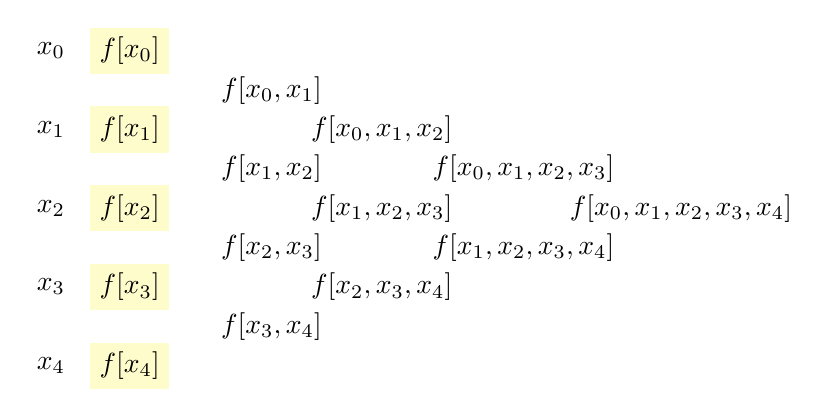
\begin{tikzpicture}
\node[] at (-1,5) {$x_0$}; \node[] at (-1,4) {$x_1$}; \node[] at (-1,3) {$x_2$}; \node[] at (-1,2) {$x_3$}; \node[] at (-1,1) {$x_4$};
\node[fill=yellow!20] at (0,5) {$f[x_0]$};
\node[fill=yellow!20] at (0,4) {$f[x_1]$};
\node[fill=yellow!20] at (0,3) {$f[x_2]$};
\node[fill=yellow!20] at (0,2) {$f[x_3]$};
\node[fill=yellow!20] at (0,1) {$f[x_4]$};
\node[] at (1.8,4.5) {$f[x_0,x_1]$};
\node[] at (1.8,3.5) {$f[x_1,x_2]$};
\node[] at (1.8,2.5) {$f[x_2,x_3]$};
\node[] at (1.8,1.5) {$f[x_3,x_4]$};
\node[] at (3.2,4) {$f[x_0,x_1,x_2]$};
\node[] at (3.2,3) {$f[x_1,x_2,x_3]$};
\node[] at (3.2,2) {$f[x_2,x_3,x_4]$};
\node[] at (5,3.5) {$f[x_0,x_1,x_2,x_3]$};
\node[] at (5,2.5) {$f[x_1,x_2,x_3,x_4]$};
\node[] at (7,3) {$f[x_0,x_1,x_2,x_3,x_4]$};
\end{tikzpicture}}
\frame{\frametitle{\ifita Complessit\`a spaziale da $O(n^2)$ a $O((n)$ \else Space Complexity from $O(n^2)$ to $O(n)$ \fi}
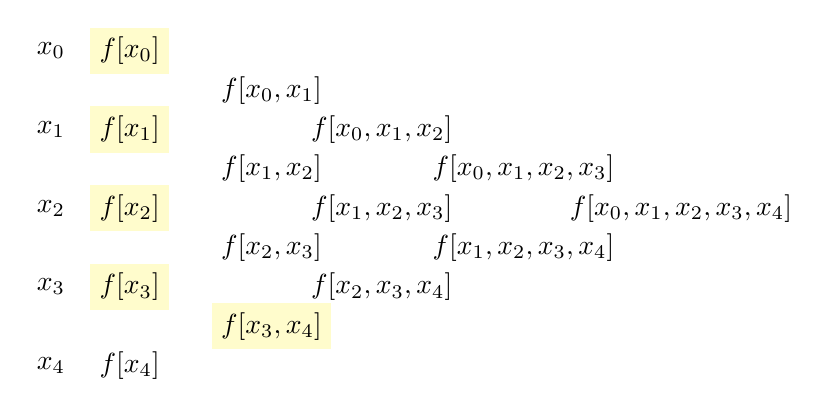
\begin{tikzpicture}
\node[] at (-1,5) {$x_0$}; \node[] at (-1,4) {$x_1$}; \node[] at (-1,3) {$x_2$}; \node[] at (-1,2) {$x_3$}; \node[] at (-1,1) {$x_4$};
\node[fill=yellow!20] at (0,5) {$f[x_0]$};
\node[fill=yellow!20] at (0,4) {$f[x_1]$};
\node[fill=yellow!20] at (0,3) {$f[x_2]$};
\node[fill=yellow!20] at (0,2) {$f[x_3]$};
\node[] at (0,1) {$f[x_4]$};
\node[] at (1.8,4.5) {$f[x_0,x_1]$};
\node[] at (1.8,3.5) {$f[x_1,x_2]$};
\node[] at (1.8,2.5) {$f[x_2,x_3]$};
\node[fill=yellow!20] at (1.8,1.5) {$f[x_3,x_4]$};
\node[] at (3.2,4) {$f[x_0,x_1,x_2]$};
\node[] at (3.2,3) {$f[x_1,x_2,x_3]$};
\node[] at (3.2,2) {$f[x_2,x_3,x_4]$};
\node[] at (5,3.5) {$f[x_0,x_1,x_2,x_3]$};
\node[] at (5,2.5) {$f[x_1,x_2,x_3,x_4]$};
\node[] at (7,3) {$f[x_0,x_1,x_2,x_3,x_4]$};
\end{tikzpicture}}

\frame{\frametitle{\ifita Complessit\`a spaziale da $O(n^2)$ a $O((n)$ \else Space Complexity from $O(n^2)$ to $O(n)$ \fi}
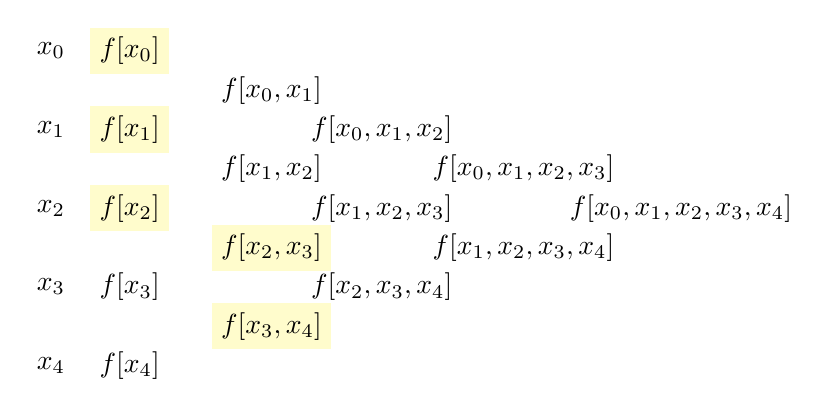
\begin{tikzpicture}
\node[] at (-1,5) {$x_0$}; \node[] at (-1,4) {$x_1$}; \node[] at (-1,3) {$x_2$}; \node[] at (-1,2) {$x_3$}; \node[] at (-1,1) {$x_4$};
\node[fill=yellow!20] at (0,5) {$f[x_0]$};
\node[fill=yellow!20] at (0,4) {$f[x_1]$};
\node[fill=yellow!20] at (0,3) {$f[x_2]$};
\node[] at (0,2) {$f[x_3]$};
\node[] at (0,1) {$f[x_4]$};
\node[] at (1.8,4.5) {$f[x_0,x_1]$};
\node[] at (1.8,3.5) {$f[x_1,x_2]$};
\node[fill=yellow!20] at (1.8,2.5) {$f[x_2,x_3]$};
\node[fill=yellow!20] at (1.8,1.5) {$f[x_3,x_4]$};
\node[] at (3.2,4) {$f[x_0,x_1,x_2]$};
\node[] at (3.2,3) {$f[x_1,x_2,x_3]$};
\node[] at (3.2,2) {$f[x_2,x_3,x_4]$};
\node[] at (5,3.5) {$f[x_0,x_1,x_2,x_3]$};
\node[] at (5,2.5) {$f[x_1,x_2,x_3,x_4]$};
\node[] at (7,3) {$f[x_0,x_1,x_2,x_3,x_4]$};
\end{tikzpicture}}

\frame{\frametitle{\ifita Complessit\`a spaziale da $O(n^2)$ a $O((n)$ \else Space Complexity from $O(n^2)$ to $O(n)$ \fi}
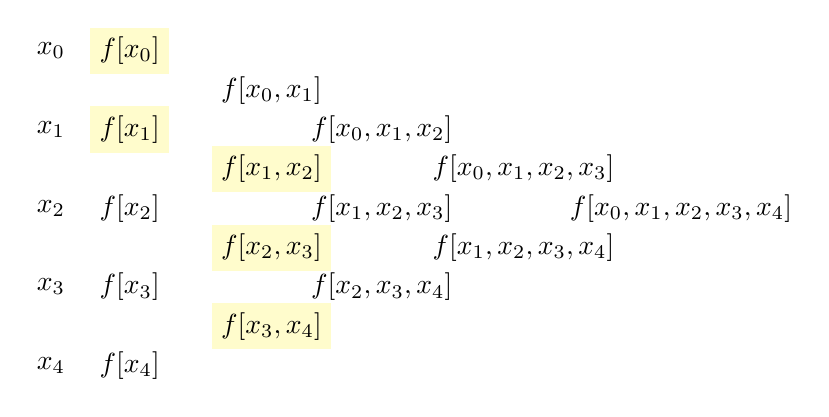
\begin{tikzpicture}
\node[] at (-1,5) {$x_0$}; \node[] at (-1,4) {$x_1$}; \node[] at (-1,3) {$x_2$}; \node[] at (-1,2) {$x_3$}; \node[] at (-1,1) {$x_4$};
\node[fill=yellow!20] at (0,5) {$f[x_0]$};
\node[fill=yellow!20] at (0,4) {$f[x_1]$};
\node[] at (0,3) {$f[x_2]$};
\node[] at (0,2) {$f[x_3]$};
\node[] at (0,1) {$f[x_4]$};
\node[] at (1.8,4.5) {$f[x_0,x_1]$};
\node[fill=yellow!20] at (1.8,3.5) {$f[x_1,x_2]$};
\node[fill=yellow!20] at (1.8,2.5) {$f[x_2,x_3]$};
\node[fill=yellow!20] at (1.8,1.5) {$f[x_3,x_4]$};
\node[] at (3.2,4) {$f[x_0,x_1,x_2]$};
\node[] at (3.2,3) {$f[x_1,x_2,x_3]$};
\node[] at (3.2,2) {$f[x_2,x_3,x_4]$};
\node[] at (5,3.5) {$f[x_0,x_1,x_2,x_3]$};
\node[] at (5,2.5) {$f[x_1,x_2,x_3,x_4]$};
\node[] at (7,3) {$f[x_0,x_1,x_2,x_3,x_4]$};
\end{tikzpicture}}

\frame{\frametitle{\ifita Complessit\`a spaziale da $O(n^2)$ a $O((n)$ \else Space Complexity from $O(n^2)$ to $O(n)$ \fi}
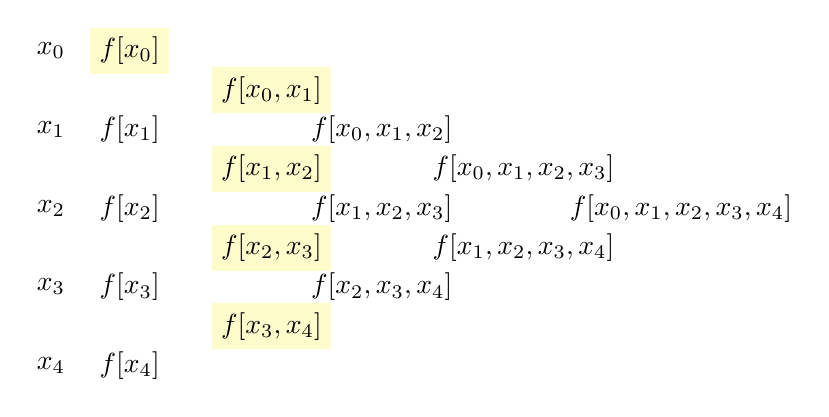
\begin{tikzpicture}
\node[] at (-1,5) {$x_0$}; \node[] at (-1,4) {$x_1$}; \node[] at (-1,3) {$x_2$}; \node[] at (-1,2) {$x_3$}; \node[] at (-1,1) {$x_4$};
\node[fill=yellow!20] at (0,5) {$f[x_0]$};
\node[] at (0,4) {$f[x_1]$};
\node[] at (0,3) {$f[x_2]$};
\node[] at (0,2) {$f[x_3]$};
\node[] at (0,1) {$f[x_4]$};
\node[fill=yellow!20] at (1.8,4.5) {$f[x_0,x_1]$};
\node[fill=yellow!20] at (1.8,3.5) {$f[x_1,x_2]$};
\node[fill=yellow!20] at (1.8,2.5) {$f[x_2,x_3]$};
\node[fill=yellow!20] at (1.8,1.5) {$f[x_3,x_4]$};
\node[] at (3.2,4) {$f[x_0,x_1,x_2]$};
\node[] at (3.2,3) {$f[x_1,x_2,x_3]$};
\node[] at (3.2,2) {$f[x_2,x_3,x_4]$};
\node[] at (5,3.5) {$f[x_0,x_1,x_2,x_3]$};
\node[] at (5,2.5) {$f[x_1,x_2,x_3,x_4]$};
\node[] at (7,3) {$f[x_0,x_1,x_2,x_3,x_4]$};
\end{tikzpicture}}


\frame{\frametitle{\ifita Complessit\`a spaziale da $O(n^2)$ a $O((n)$ \else Space Complexity from $O(n^2)$ to $O(n)$ \fi}
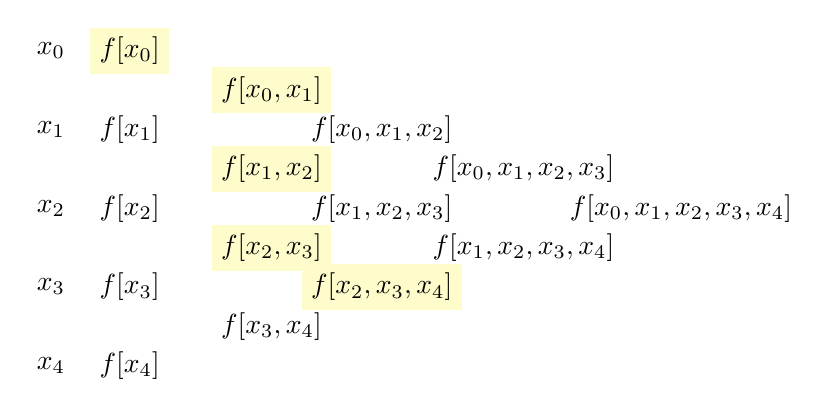
\begin{tikzpicture}
\node[] at (-1,5) {$x_0$}; \node[] at (-1,4) {$x_1$}; \node[] at (-1,3) {$x_2$}; \node[] at (-1,2) {$x_3$}; \node[] at (-1,1) {$x_4$};
\node[fill=yellow!20] at (0,5) {$f[x_0]$};
\node[] at (0,4) {$f[x_1]$};
\node[] at (0,3) {$f[x_2]$};
\node[] at (0,2) {$f[x_3]$};
\node[] at (0,1) {$f[x_4]$};
\node[fill=yellow!20] at (1.8,4.5) {$f[x_0,x_1]$};
\node[fill=yellow!20] at (1.8,3.5) {$f[x_1,x_2]$};
\node[fill=yellow!20] at (1.8,2.5) {$f[x_2,x_3]$};
\node[] at (1.8,1.5) {$f[x_3,x_4]$};
\node[] at (3.2,4) {$f[x_0,x_1,x_2]$};
\node[] at (3.2,3) {$f[x_1,x_2,x_3]$};
\node[fill=yellow!20] at (3.2,2) {$f[x_2,x_3,x_4]$};
\node[] at (5,3.5) {$f[x_0,x_1,x_2,x_3]$};
\node[] at (5,2.5) {$f[x_1,x_2,x_3,x_4]$};
\node[] at (7,3) {$f[x_0,x_1,x_2,x_3,x_4]$};
\end{tikzpicture}}

\frame{\frametitle{\ifita Complessit\`a spaziale da $O(n^2)$ a $O((n)$ \else Space Complexity from $O(n^2)$ to $O(n)$ \fi}
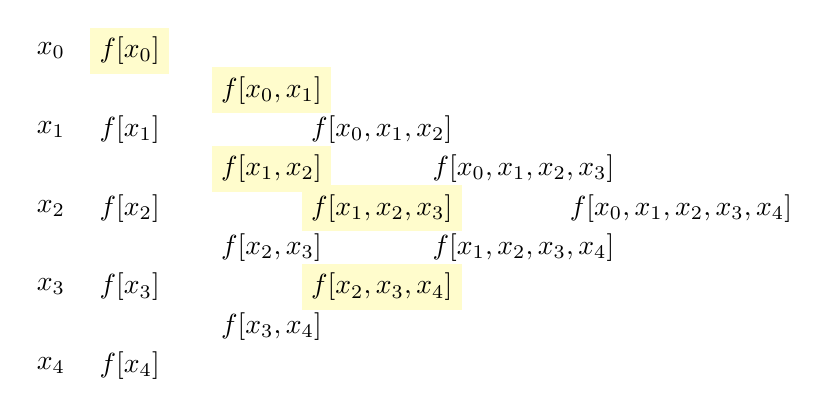
\begin{tikzpicture}
\node[] at (-1,5) {$x_0$}; \node[] at (-1,4) {$x_1$}; \node[] at (-1,3) {$x_2$}; \node[] at (-1,2) {$x_3$}; \node[] at (-1,1) {$x_4$};
\node[fill=yellow!20] at (0,5) {$f[x_0]$};
\node[] at (0,4) {$f[x_1]$};
\node[] at (0,3) {$f[x_2]$};
\node[] at (0,2) {$f[x_3]$};
\node[] at (0,1) {$f[x_4]$};
\node[fill=yellow!20] at (1.8,4.5) {$f[x_0,x_1]$};
\node[fill=yellow!20] at (1.8,3.5) {$f[x_1,x_2]$};
\node[] at (1.8,2.5) {$f[x_2,x_3]$};
\node[] at (1.8,1.5) {$f[x_3,x_4]$};
\node[] at (3.2,4) {$f[x_0,x_1,x_2]$};
\node[fill=yellow!20] at (3.2,3) {$f[x_1,x_2,x_3]$};
\node[fill=yellow!20] at (3.2,2) {$f[x_2,x_3,x_4]$};
\node[] at (5,3.5) {$f[x_0,x_1,x_2,x_3]$};
\node[] at (5,2.5) {$f[x_1,x_2,x_3,x_4]$};
\node[] at (7,3) {$f[x_0,x_1,x_2,x_3,x_4]$};
\end{tikzpicture}}

\frame{\frametitle{\ifita Complessit\`a spaziale da $O(n^2)$ a $O((n)$ \else Space Complexity from $O(n^2)$ to $O(n)$ \fi}
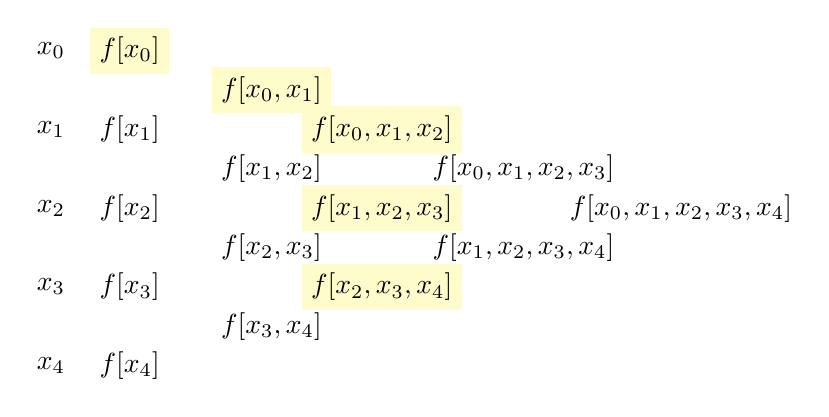
\begin{tikzpicture}
\node[] at (-1,5) {$x_0$}; \node[] at (-1,4) {$x_1$}; \node[] at (-1,3) {$x_2$}; \node[] at (-1,2) {$x_3$}; \node[] at (-1,1) {$x_4$};
\node[fill=yellow!20] at (0,5) {$f[x_0]$};
\node[] at (0,4) {$f[x_1]$};
\node[] at (0,3) {$f[x_2]$};
\node[] at (0,2) {$f[x_3]$};
\node[] at (0,1) {$f[x_4]$};
\node[fill=yellow!20] at (1.8,4.5) {$f[x_0,x_1]$};
\node[] at (1.8,3.5) {$f[x_1,x_2]$};
\node[] at (1.8,2.5) {$f[x_2,x_3]$};
\node[] at (1.8,1.5) {$f[x_3,x_4]$};
\node[fill=yellow!20] at (3.2,4) {$f[x_0,x_1,x_2]$};
\node[fill=yellow!20] at (3.2,3) {$f[x_1,x_2,x_3]$};
\node[fill=yellow!20] at (3.2,2) {$f[x_2,x_3,x_4]$};
\node[] at (5,3.5) {$f[x_0,x_1,x_2,x_3]$};
\node[] at (5,2.5) {$f[x_1,x_2,x_3,x_4]$};
\node[] at (7,3) {$f[x_0,x_1,x_2,x_3,x_4]$};
\end{tikzpicture}}

\frame{\frametitle{\ifita Complessit\`a spaziale da $O(n^2)$ a $O((n)$ \else Space Complexity from $O(n^2)$ to $O(n)$ \fi}
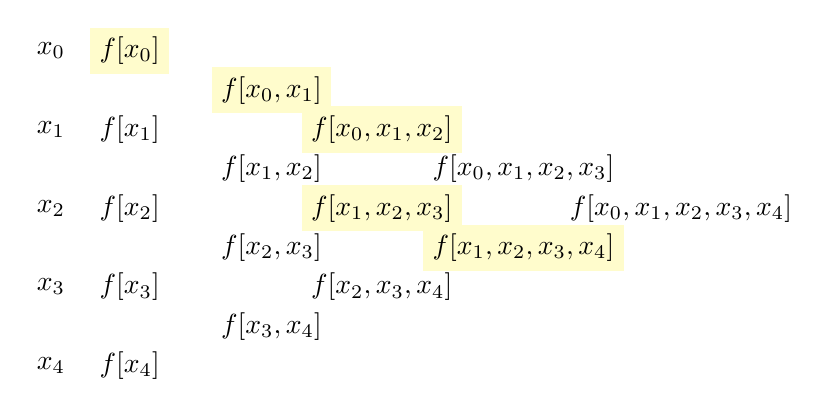
\begin{tikzpicture}
\node[] at (-1,5) {$x_0$}; \node[] at (-1,4) {$x_1$}; \node[] at (-1,3) {$x_2$}; \node[] at (-1,2) {$x_3$}; \node[] at (-1,1) {$x_4$};
\node[fill=yellow!20] at (0,5) {$f[x_0]$};
\node[] at (0,4) {$f[x_1]$};
\node[] at (0,3) {$f[x_2]$};
\node[] at (0,2) {$f[x_3]$};
\node[] at (0,1) {$f[x_4]$};
\node[fill=yellow!20] at (1.8,4.5) {$f[x_0,x_1]$};
\node[] at (1.8,3.5) {$f[x_1,x_2]$};
\node[] at (1.8,2.5) {$f[x_2,x_3]$};
\node[] at (1.8,1.5) {$f[x_3,x_4]$};
\node[fill=yellow!20] at (3.2,4) {$f[x_0,x_1,x_2]$};
\node[fill=yellow!20] at (3.2,3) {$f[x_1,x_2,x_3]$};
\node[] at (3.2,2) {$f[x_2,x_3,x_4]$};
\node[] at (5,3.5) {$f[x_0,x_1,x_2,x_3]$};
\node[fill=yellow!20] at (5,2.5) {$f[x_1,x_2,x_3,x_4]$};
\node[] at (7,3) {$f[x_0,x_1,x_2,x_3,x_4]$};
\end{tikzpicture}}

\frame{\frametitle{\ifita Complessit\`a spaziale da $O(n^2)$ a $O((n)$ \else Space Complexity from $O(n^2)$ to $O(n)$ \fi}
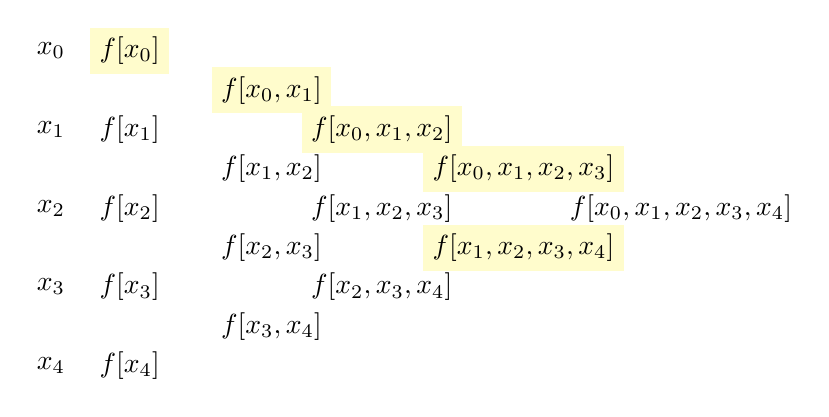
\begin{tikzpicture}
\node[] at (-1,5) {$x_0$}; \node[] at (-1,4) {$x_1$}; \node[] at (-1,3) {$x_2$}; \node[] at (-1,2) {$x_3$}; \node[] at (-1,1) {$x_4$};
\node[fill=yellow!20] at (0,5) {$f[x_0]$};
\node[] at (0,4) {$f[x_1]$};
\node[] at (0,3) {$f[x_2]$};
\node[] at (0,2) {$f[x_3]$};
\node[] at (0,1) {$f[x_4]$};
\node[fill=yellow!20] at (1.8,4.5) {$f[x_0,x_1]$};
\node[] at (1.8,3.5) {$f[x_1,x_2]$};
\node[] at (1.8,2.5) {$f[x_2,x_3]$};
\node[] at (1.8,1.5) {$f[x_3,x_4]$};
\node[fill=yellow!20] at (3.2,4) {$f[x_0,x_1,x_2]$};
\node[] at (3.2,3) {$f[x_1,x_2,x_3]$};
\node[] at (3.2,2) {$f[x_2,x_3,x_4]$};
\node[fill=yellow!20] at (5,3.5) {$f[x_0,x_1,x_2,x_3]$};
\node[fill=yellow!20] at (5,2.5) {$f[x_1,x_2,x_3,x_4]$};
\node[] at (7,3) {$f[x_0,x_1,x_2,x_3,x_4]$};
\end{tikzpicture}}


\frame{\frametitle{\ifita Complessit\`a spaziale da $O(n^2)$ a $O((n)$ \else Space Complexity from $O(n^2)$ to $O(n)$ \fi}
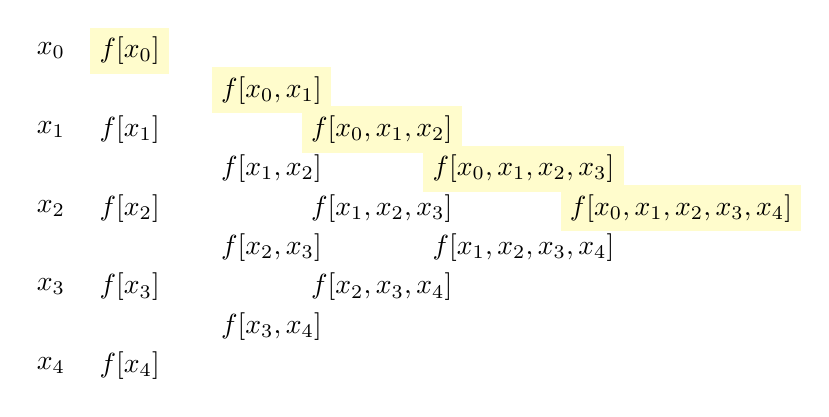
\begin{tikzpicture}
\node[] at (-1,5) {$x_0$}; \node[] at (-1,4) {$x_1$}; \node[] at (-1,3) {$x_2$}; \node[] at (-1,2) {$x_3$}; \node[] at (-1,1) {$x_4$};
\node[fill=yellow!20] at (0,5) {$f[x_0]$};
\node[] at (0,4) {$f[x_1]$};
\node[] at (0,3) {$f[x_2]$};
\node[] at (0,2) {$f[x_3]$};
\node[] at (0,1) {$f[x_4]$};
\node[fill=yellow!20] at (1.8,4.5) {$f[x_0,x_1]$};
\node[] at (1.8,3.5) {$f[x_1,x_2]$};
\node[] at (1.8,2.5) {$f[x_2,x_3]$};
\node[] at (1.8,1.5) {$f[x_3,x_4]$};
\node[fill=yellow!20] at (3.2,4) {$f[x_0,x_1,x_2]$};
\node[] at (3.2,3) {$f[x_1,x_2,x_3]$};
\node[] at (3.2,2) {$f[x_2,x_3,x_4]$};
\node[fill=yellow!20] at (5,3.5) {$f[x_0,x_1,x_2,x_3]$};
\node[] at (5,2.5) {$f[x_1,x_2,x_3,x_4]$};
\node[fill=yellow!20] at (7,3) {$f[x_0,x_1,x_2,x_3,x_4]$};
\end{tikzpicture}
\begin{itemize}
\item \ifita Posso  "far stare" i conti in un vettore di lunghezza 5!
\else
Storing all the computations in a list of size 5!
\fi
\end{itemize}

}























\end{document}
